\chapter{Návrh vlastnej analýzy}
\label{possible-analysis-strategies}

% \subsubsection{Úvod}

V tejto kapitole popisujem návrh na vypracovanie vlastnej analázy spojenej s technológiou NEL.
Najskôr predstavujem rozsah a uplatnenie tejto práce rozdelenej do troch častí, ktorými som sa rozhodol zaoberať.
Potom prechádzam k spôsobom, akými jednotlivé časti navrhujem vypracovať.
Nakoniec zdôvodňujem svoje návrhy v záverečnej diskuzií pred ich implementáciou.

\subsubsection{Definícia čiastkových úloh}

Mojou prácou je analyzovať využívanie technológie NEL (viď kapitola \ref{nel-and-related-technologies}) pomocou dostupných metód a nástrojov.
Dôležitá je pri tom relevantnosť vypracovanej analýzy.
Prečítaním existujúcich prác (viď kapitola \ref{related-work}), ktorých zameraním bol rovnako NEL, som zistil, že bol NEL za určité obdobie už skúmaný.
Preto je predovšetkým nutné si vybrať počiatočný dátum, od ktorého budem informácie o nasadení NEL hľadať. 
Výberom vhodného dátumu je mi sprístupnená možnosť nadviazať na predošlé práce a porovnať si s nimi výsledky.
Porovnávanie výsledkov však má zmysel iba v prípade, že vynaložím úsilie čo najviac replikovať zoznam skúmaných domén použitý ako vstup pre spomínané predošlé práce.
Preto je po výbere dátumu ďalším krokom vybrať taktiež vhodné vstupy pre moju vlastnú analýzu.
Vstupy tu predstavujú zoznamy domén potrebné pre definíciu skúmanej množiny web serverov, na ktorých sa NEL využíva.
Tieto zoznamy sú v podobe rebríčkov populárnosti spomínané v kapitole \ref{data-sources-available-for-research}.
Vďaka predošlým skúsenostiam, ktoré nadobudli záujemci o NEL v ich odborných prácach, viem, že nasadenie NEL na webe je možné sledovať viacerými spôsobmi.
Zvoliť si vhodný spôsob spomedzi nich sa dá po určení, či chcem skúmať aktuálne dáta alebo záznamy z minulosti.
Po výbere vstupov a získaní relevantných dát je analýza v poslednom bode, a to bode týkajúceho sa prezentácie výsledkov.
Inšpiráciou vhodnej formy prezentácie môže byť napríklad report Web Almanac spomínaný v sekcii \ref{web-almanac}.
Podľa v ňom zahrnutých hlásení o jednotlivých technológiach na webe je možné štruktúrovať aj moju vlastnú analýzu.
Výsledkom teda môže byť sada grafických vizualizácií zisteného stavu využitia NEL počas skúmanej doby a k nim pridaný dodatočný popis konkrétnych metrík, na ktoré sa rozhodnem zamerať.

\pagebreak

\begin{figure}[!htb]
\begin{center}
 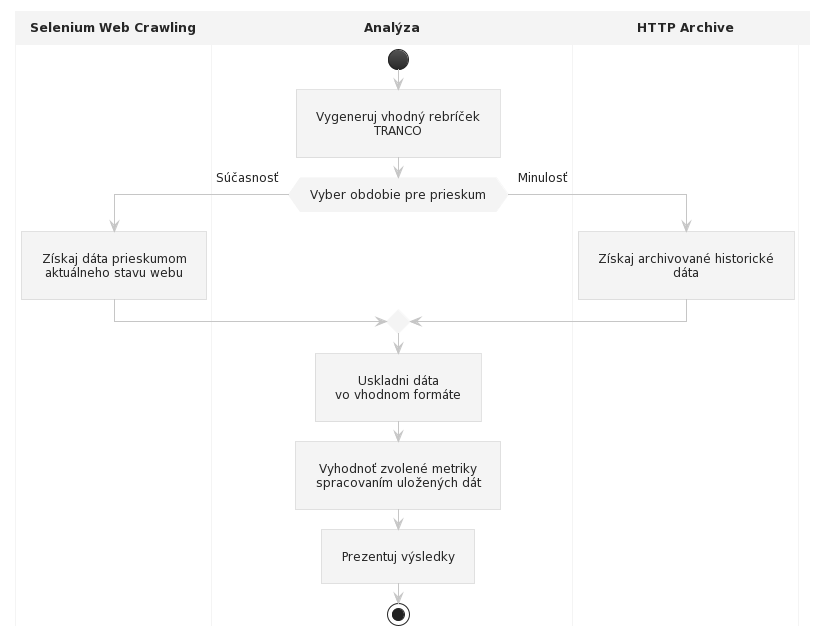
\includegraphics[scale=0.48]{obrazky-figures/analysis-activity-diagram.png}    
 \caption{\centering Rozdelenie analýzy na čiastkové úlohy. Celková analýza môže byť vykonaná v krokoch uvedených na obrázku. Dôležité kroky sú najmä generovanie rebríčka, výber spôsobu získania dát a ich prezentácia. Ideálnym výsledkom práce je vytvoriť nástroj, ktorý tieto aktivity automatizuje (viď záver tejto kapitoly).}
 \label{img:analysis-activity-diagram}
\end{center}
\end{figure}

\subsubsection{Stratégia výberu zoznamu domén}

Pri vyberaní vstupov pre analýzu som sa rozhodol nedržať sa predošlých podobných prác.
Navrhol som radšej sa pokúsiť o vygenerovanie takého zoznamu domén, ktorý bude obsahovať domény 
s vysokou pravdepodobnosťou výskytu hlavičky NEL. 
To znamená, že sa zameriam na vytvorenie zoznamu obsahujúceho domény s vysokou návštevnosťou, ktoré sa v udržiavajú vysoko v rebríčkoch populárnosti už dlhšiu dobu.
Ďalej, v rámci konfigurácie generovania nového zoznamu nebudem zakomponovávať žiadne subdomény.
To z takého dôvodu, že sa zameriavam na najdôležitejšie domény, kde by mala byť žiadanosť 
monitorovania poskytovaných zdrojov najvyššia.
Použíté rebríčky teda môžu byť napríklad: Chrome User Experience Report a Cloudflare Radar.
Ak by som však zistil, že výsledný vygenerovaný rebríček nespĺňa očakávania, zmenil by som buď zoznam zdrojových rebríčkov
V prípade, že by výsledky aj po otestovaní rôznych kombinácií zdrojových rebríčkov nevykazovali očakávané výsledky, ako zámenu využijem zoznam verejných suffixov (viď \mbox{sekciu \ref{public-suffix-and-etld})}.

\subsubsection{Výber skúmaných období}

V mojej analýze som sa rozhodol zahrnúť ako stav aktuálny, tak aj historický.
Z hladiska histórie rešpektujem posledný dátum skúmania využitia technológie NEL (viď sekciu \ref{praca-veduceho}).
Preto som si \textbf{vybral rok 2023} ako vhodné obdobie pre sledovanie nasadenia NEL na webe pre vybrané domény.

Čo sa aktuálneho stavu týka, navrhol som \textbf{nástroj pre prieskum} webu formou Web Crawling.
Tento nástroj bude mať za úlohu skúmať stav \textbf{v reálnom čase}.

\subsubsection{Nástroje pre analýzu}

Pre analýzu stavu za rok 2023 použijem archivované dáta projektom \textbf{HTTP Archive}, ktoré sú dostupné na Google Cloud Platform (GCP).
Na spracovanie týchto dát použijem už \textbf{existujúci skript} od pána Ing. Kamila Jeřábka. 
Tento skript bol použitý v rámci predošlej analýzy využitia NEL v roku 2022 (viď sekciu \ref{skript}).
Jeho funkciou je sťahovať dáta z GCP a ukladať ich vo vhodnom formáte pre ďalšie spracovanie.
V prípade, že by tento skript bol zastaraný ho upravím a otestujem nanovo.

Pre analýzu aktuálneho stavu použijem mnou navrhnutý nástroj pre Web Crawling. 
Vstupom pre tento nástroj (aspoň v mojej analýze) bude rovnaký rebríček domén, 
aký použijem aj na prieskum stavu z archivovaných dát.
Jeho úlohou bude vytvoriť spojenie s web servermi týchto domén a detegovať hlavičky NEL pri HTTPS prenose na nimi poskytovaných zdrojoch.
Taktiež by mal byť schopný v prípade získania webstránok skúmať aj hyperlinky v rámci obsahu ich HTML kódu.
Išlo by o rozšírenie tohto nástroja pre \textbf{detekciu hlavičiek NEL aj na pod-stránkach} uložených na jednej doméne (nie iba na domovskej stránke).
Cieľom by bolo získať kompletný prehľad o využití NEL na danej doméne, \textbf{čo projekt HTTP Archive nedokáže} z dôvodu, že skúma iba domovské stránky. 
Špecifickým výstupom môjho nástroja budú dáta uložené vo vhodnom formáte pre ďalšie spracovanie.


\subsubsection{Výsledky}

K výsledkom celkovej vlastnej analýzy sa dopracujem spracovaním uložených aktuálnych a historických dát získaných použitím vyššie uvedených nástrojov.
Zameriam sa primárne na získanie metrík celkového využitia NEL, jeho populárnych konfigurácií a monitorovaciu pokrytosť pod-stránok na konkrétnej doméne.


\subsubsection{Pridaná hodnota}

V rámci tejto práce som sa taktiež rozhodol vytvoriť balík funkcií, ktoré výsledné metriky spomenuté vyššie (a prípadne aj ďalšie) budú graficky vizualizovať.
Vizualizáciou získaných metrík sa chcem priblížiť k štýlu hlásenia z prieskumu, akým je práve Web Almanac (uvedený v sekcií \ref{web-almanac}).
V prípade úspešného vypracovania tejto časti som navrhol spojiť sa s autormi Web Almanac a pokúsiť sa pridať výsledky tejto práce ako samostatné nové hlásenie o stave webu do ďalšieho Web Almanac reportu. 
